%%%%%%%%%%%%%%%%%%%%%%%%%%%%%%%%%%%%
% Header                           %
%%%%%%%%%%%%%%%%%%%%%%%%%%%%%%%%%%%%
% 
% Revisions: 2017-04-10 Martin R�del <martin.raedel@dlr.de>
%                       Initial draft
%               
% Contact:   Martin R�del,  martin.raedel@dlr.de
%            DLR Composite Structures and Adaptive Systems
%          
%                                 __/|__
%                                /_/_/_/  
%            www.dlr.de/fa/en      |/ DLR
% 
%%%%%%%%%%%%%%%%%%%%%%%%%%%%%%%%%%%%
% Content                          %
%%%%%%%%%%%%%%%%%%%%%%%%%%%%%%%%%%%%

\levelstay{Node/point distance}

\begin{figure}[htbp]
\centering
  \begin{tikzpicture}
    % External figure
    \node[anchor=south west,inner sep=0] (image) at (0,0) {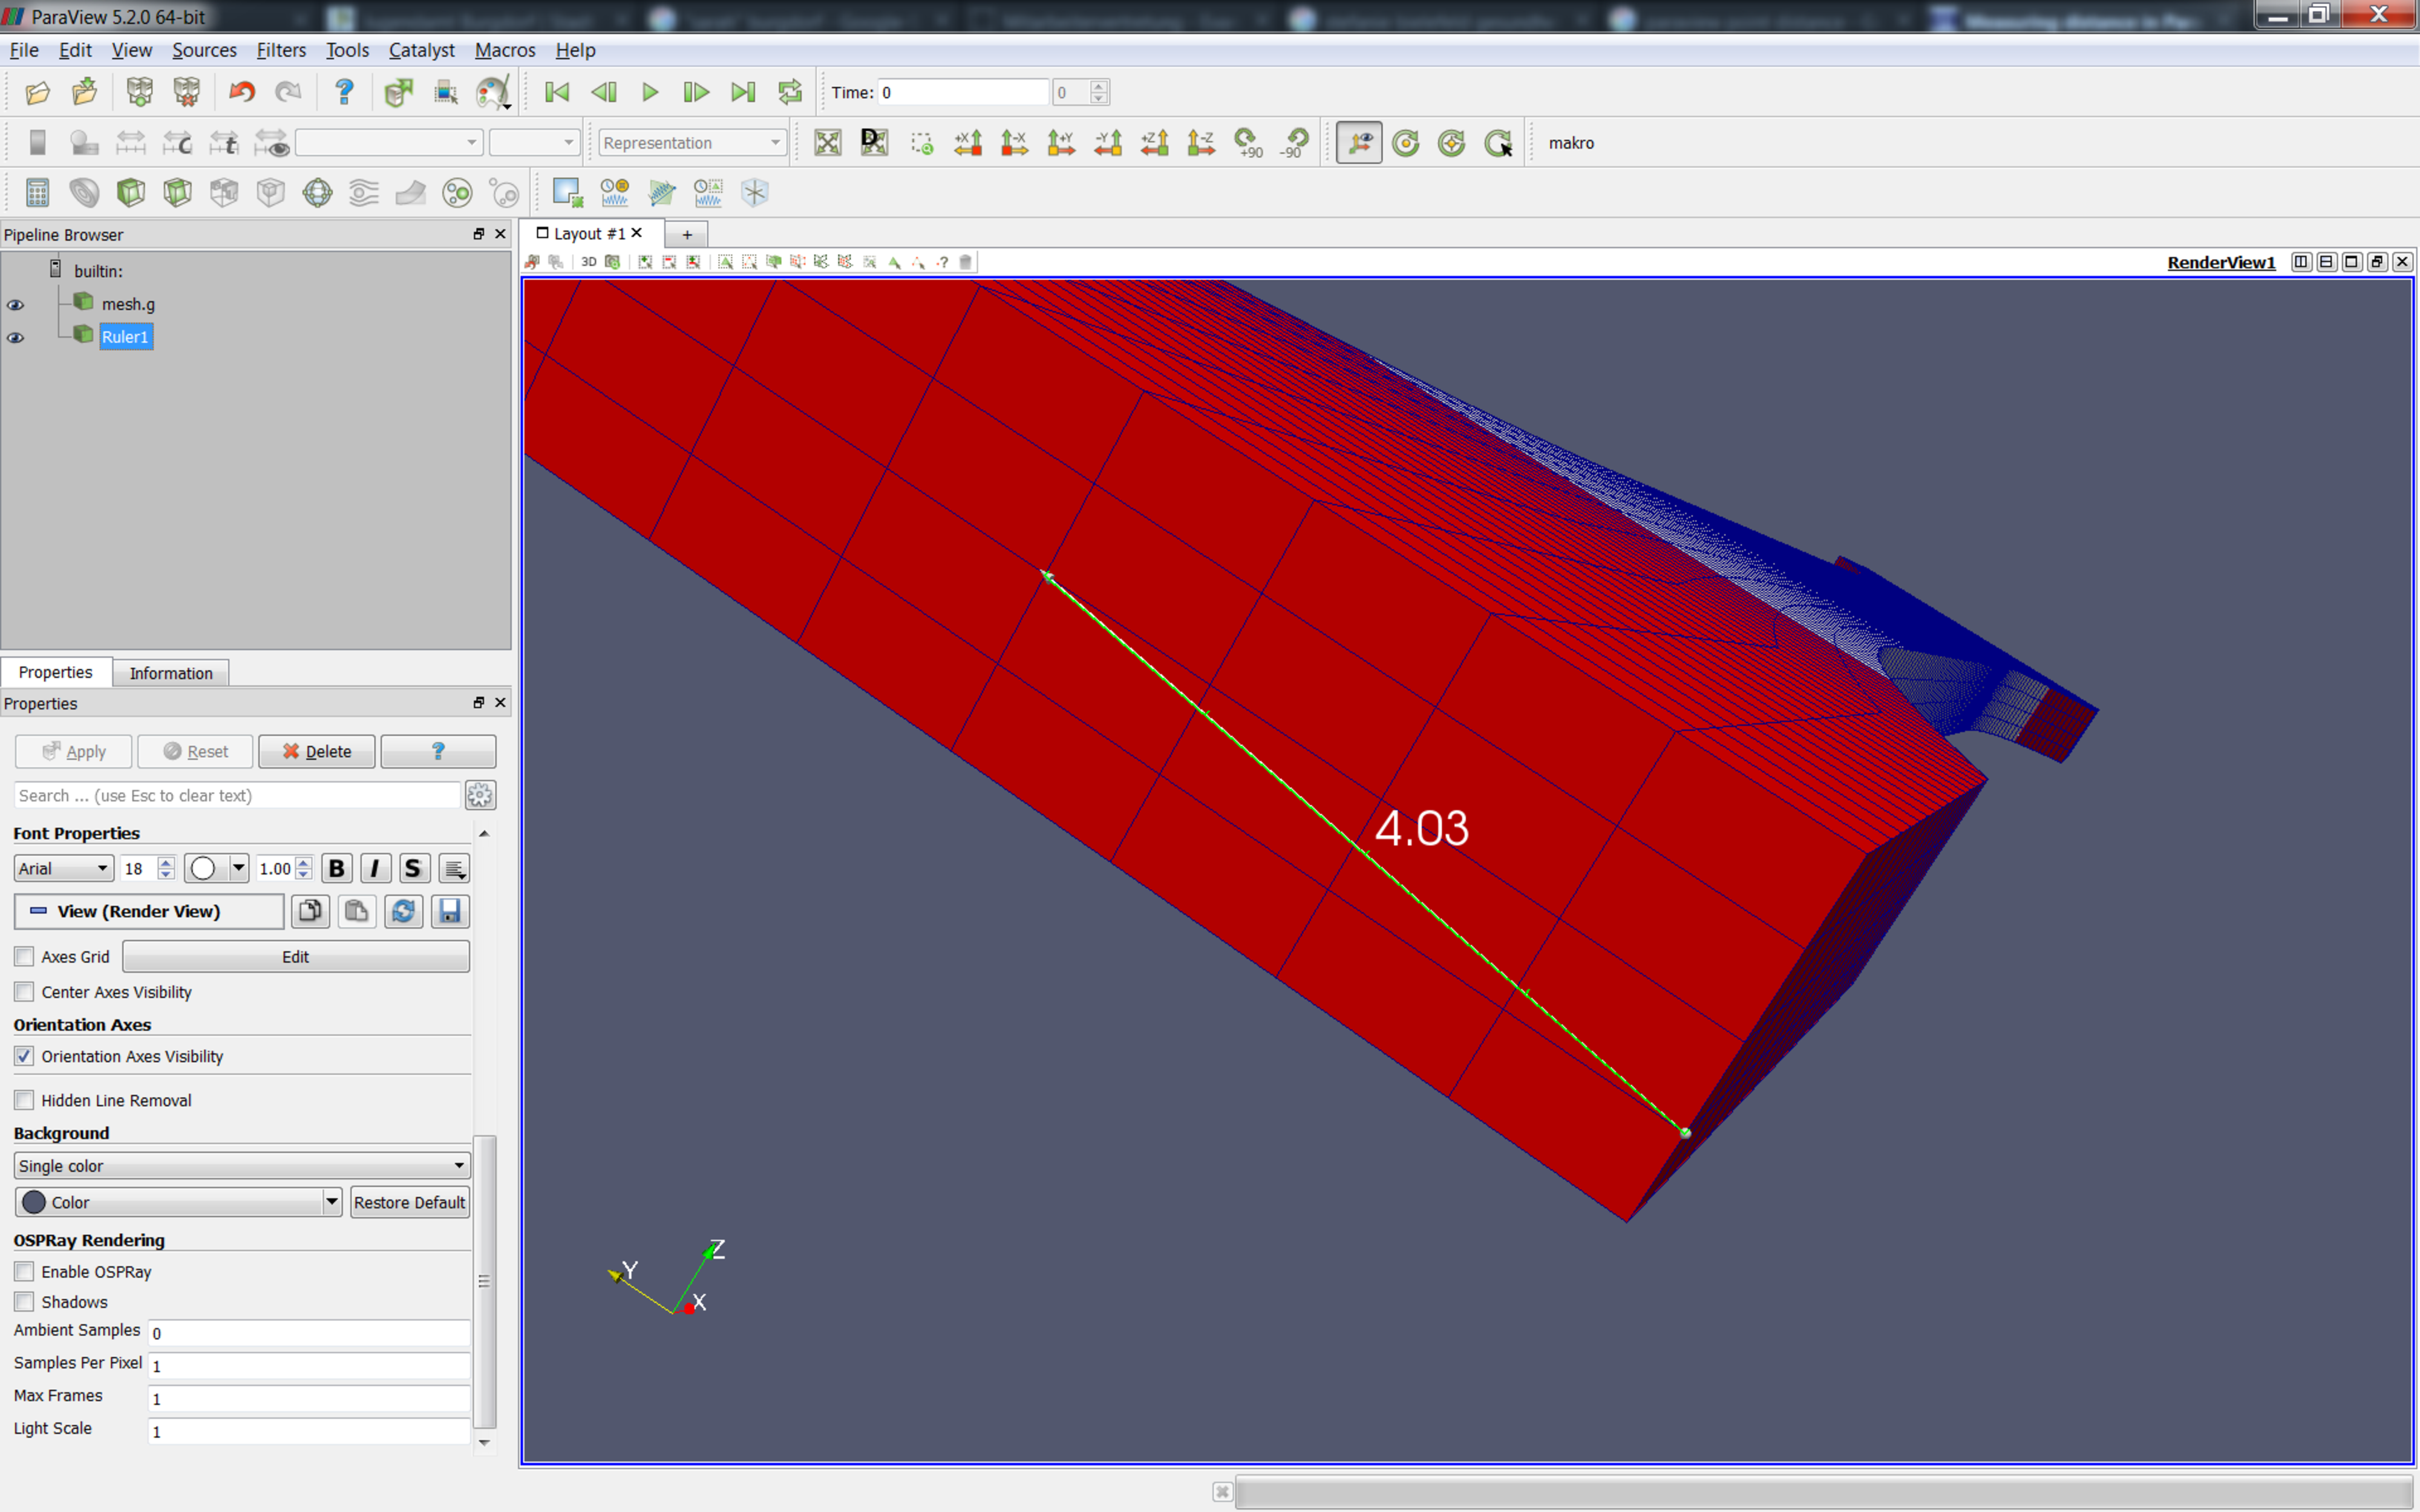
\includegraphics[width=\paraviewscreenshotwidthfac\linewidth]{Figures/Screenshots/ParaView_Measure_NodeDistance}};
    \begin{scope}[
      x={(image.south east)},
      y={(image.north west)},
    ]
      % Some label
%         \node[fit={(0.007,0.10) (0.18,0.17)},myrectangularmarkup] (rect1) {};
%         \node[anchor=west,mymarkuptext] (rect1label) at (rect1.east) {1};
%         %
%         \node[fit={(0.280,0.83) (0.31,0.86)},myrectangularmarkup] (rect2) {};
%         \node[anchor=west,mymarkuptext] (rect2label) at (rect2.east) {2};
      % Help grid and labels
%       \pic{myimagegrid};
    \end{scope}
  \end{tikzpicture}
\caption{Measure point distance in \protect\paraviewname}
\label{fig:Use_ParaView_Measure_NodeDistance}
\end{figure}

To measure the distance between two nodes or collocation points after importing the model:

\begin{enumerate}[noitemsep]
  \item In the menu bar
  \begin{itemize}[noitemsep]
    \item Click on \textit{Sources}
    \item Click \textit{Ruler}
  \end{itemize}
  \item In the render view
  \begin{itemize}[noitemsep]
    \item Left-click the first point and keep the mouse clicked
    \item Move the point close to the target
    \item Press ``CTRL+1'' and snap the point to the closest mesh point
    \item Do the same for the second point, but press ``CTRL+2'' instead for snapping
  \end{itemize}
  \item In the \textit{Ruler} properties window
  \begin{itemize}[noitemsep]
    \item Adjust preferences to your need
    \item Click \textit{Apply}
  \end{itemize}
  \item The number next to the \textit{Ruler} in the render view is the point distance
\end{enumerate}
